\section{Durchführung}
\label{sec:Durchführung}

Der Versuch wird, wie in der Abbildung \ref{fig:Ftröpfchen} aufgebaut.
\begin{figure}[H]
    \centering
    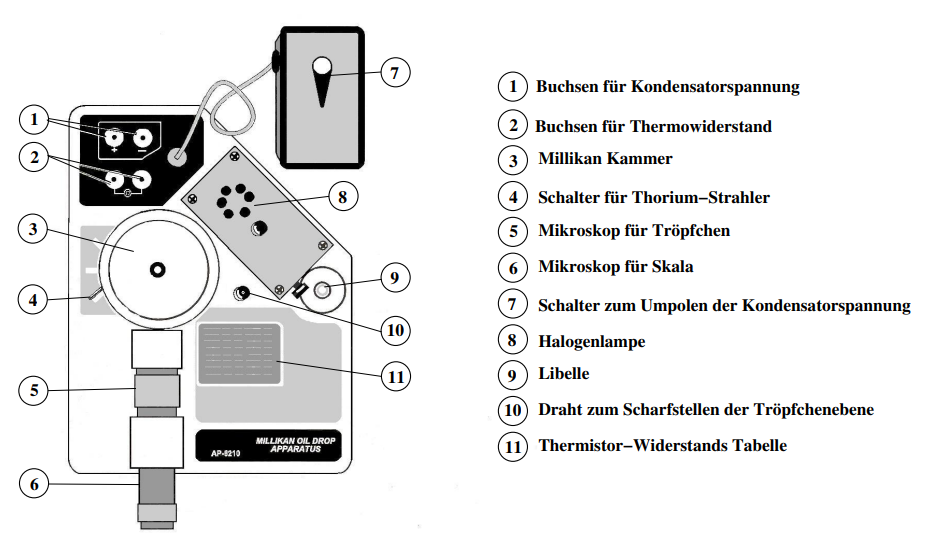
\includegraphics[scale=0.5]{content/Aufbau.png}
    \caption{Aufbau des Millikan-Versuchs.}
    \label{fig:Ftröpfchen}
\end{figure}

Es kann zusätzlich eine Kamera vor das Mikroskop gestellt werde, die das Bild dann auf einem Bildschirm anzeigt.
Um das Mikroskop scharf einzustellen, kann der Draht verwendet werden.
Wenn sich zu viel Öl im Kondensator befindet, kann es sein, dass keine Tröpfchen zu erkennen sind.
Dann kann der Kondensator mit einem Tuch gereinigt werden.
An der Öffnung wird dann der Zerstäuber gehalten und die Öltröpfchen in den Kondensator gestäubt.
Zwischen den Kondensatorplatten befindet sich Millimeterpapier, anhand dem die Strecke eines Tröpfchen abgelesen werden kann.
Es wird zunächst die am Kondensator angelegte Spannung eingestellt.
Durch das Mikroskop wird ein Tröpfchen ausgesucht mit dem die Messungen durchgeführt werden.
Wenn sich zu viele Tröpfchen im Kondensator befinden, wird kurz gewartet, bis die Tröpfchen abgesunken sind.
Mithilfe des Schalters, werden die Platten gepolt. Das Teilchen bewegt sich nach oben oder nach unten.
Es wird nun die Zeit t mithilfe einer Stoppuhr gemessen, in dem das Teilchen eine Strecke von $s = \qty{0.5}{mm}$ zurückgelegt hat.
Dann wird der Kondensator umgepolt und die Zeit wird wieder für die gleiche Strecke gemessen.
Es wird insgesamt drei mal für die Bewegung nach obne $t_\text{auf}$ und die Bewegung nach unten $t_\text{ab}$ gemessen.
Zusätzlich wird noch die Zeit $t_0$ gemessen, indem der Schalter zur Umpolung in der Mitte gestellt wird.
Diese Zeit wird nur ein mal gemessen.
Wenn alle Zeiten aufgenommen wurden, wird sich das nächste Tröpfchen ausgesucht.
Diese Messung wird für vier verschiedene Tröpfchen durchgefürhrt.
Dann wird eine andere Kondensatorspannung eingestellt und auch bei dieser werden die Zeiten für vier verschiedene Tröpfchen gemessen.
Die Spannung wird viermal varriert.
Somit werden insgesamt 16 Tröpfchen gemessen.
Zwischendurch wird noch zusätzlich die der Widerstand des Thermistors mit einem Multimeter gemessen und notiert. 
Dieser sollte sich während der Messung verändern, da die Halogenlampe die Apperatur aufheizt.
